\documentclass[12pt, twoside]{article}
\usepackage[utf8]{inputenc}
\usepackage[english]{babel}

\usepackage{amsthm}
\usepackage{a4wide}
\usepackage{graphicx}
\usepackage{caption}
\usepackage{amssymb}
\usepackage{amsmath}
\usepackage{mathrsfs}
\usepackage{euscript}
\usepackage{graphicx}
\usepackage{subfig}
\usepackage{caption}
\usepackage{color}
\usepackage{bm}
\usepackage{tabularx}
\usepackage{adjustbox}


\usepackage[toc,page]{appendix}

\usepackage{comment}
\usepackage{rotating}

\DeclareMathOperator*{\argmax}{arg\,max}
\DeclareMathOperator*{\argmin}{arg\,min}

\renewcommand{\baselinestretch}{1.35}


\numberwithin{equation}{section}

\newcommand*{\No}{No.}
\begin{document}

\title{\bf Analysis of the properties of local models in clustering problems of quasi-periodic time series\thanks{This research was supported by RFBR, project ..., and by Government of the Russian Federation, agreement ...}}
\date{}
\author{}
\maketitle

\begin{center}
\bf
A.\,V.~Grabovoy\footnote{Moscow Institute of Physics and Technology, grabovoy.av@phystech.edu}, V.\,V.~Strijov\footnote{Moscow Institute of Physics and Technology, strijov@ccas.ru}

\end{center}

{\centering\begin{quote}
\textbf{Annotation:} The paper analysis periodic signals in the time series for recognize the physical actions of a person by using a mobile accelerometer. 
The method of clustering points of the time series is proposed for searching quasi-periodic segments of the time series. 
Time series are objects of a complex structure. 
There are not any feature vector for describe points of a time series. 
The paper proposes to consider principal components of the local neighborhood of the phase trajectory near some point for feature description of this point.
The article proposes a distance function between points in the new space of objects.
Clustering is carried out using a matrix of pairwise distances between the points in time series.
The algorithm was tested on synthetic and real data. Real data was obtained by using a mobile accelerometer.


\smallskip
\textbf{Key words}: time series; clustering; segmentation; recognition of physical activity; principal component method.

\smallskip
%\textbf{DOI}: 00.00000/00000000000000
\end{quote}
}

\section{Introduction}
Analysis of a person’s physical activity is carried out by using mobile phones, smart watches etc~\cite{kwapisz2010, wang2014}.
These devices are using an accelerometer, gyroscope and magnetometer. 
The main purpose of this work is to markup and recognize human activity during the time~\cite{Ignatov2015, Olivares2012}, and also search for the beginning of a periodic signal~\cite{motrenko2015, cinar2018}.
Examples of an action segment is a step, a step of running, a single squat, a single jump, etc.
Current work considers an sequences  that consist of at least two consecutive segments that correspond to the same type of human activity.

\begin{figure}[h!t]\center
\subfloat[]
{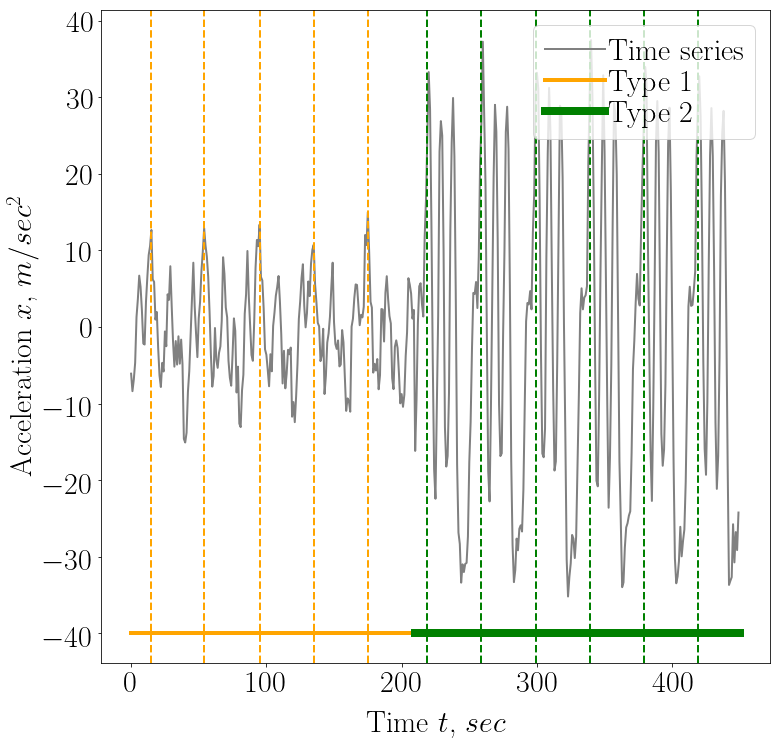
\includegraphics[width=0.5\textwidth]{results/example}\label{example:1}}
\subfloat[]
{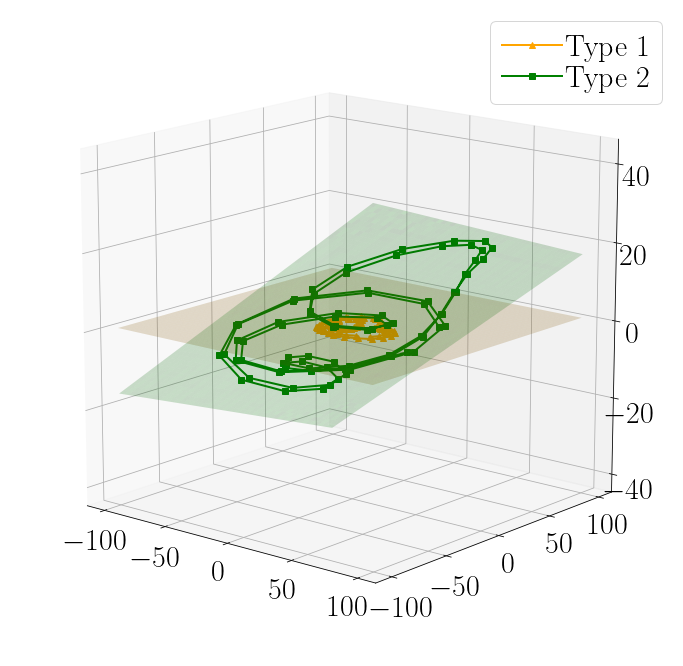
\includegraphics[width=0.5\textwidth]{results/example_phase}\label{example:2}}\\
\caption{A time series with clustering:  a) time series with assessor markings on clusters and markings at beginning of each quasi-periodic segment; b) projection of phase trajectories on the first two principal components}
\end{figure}

Time series are objects of complex structure. 
The method of constructing feature vectors for points is very important for their clustering.
In this article, the object of analysis, as well as clustering, is a point on the time axis.
The paper investigates the problem of clustering points in a time series.
\textit{Clustering} is a process in which all points in a time series are labeled with a label from the finite set of labels.
Each label corresponds to one characteristic physical action.
A \textit{segment} is a part of a time series that corresponds to one characteristic physical action, for example: a step with two legs when walking, or a step with two legs when running.
A sequence of segments that correspond to one physical action form a \textit{chain} of actions.
It is assumed that the chain of actions forms a quasi-periodic sequence of values of the time series.
A sequence of points $\{b_t\}_{t=1}^{N}$ is called \textit{quasi-periodic} with period of $T$, if for all $t$ there is a $\Delta$, such that:
\begin{equation}
\label{eq:int:1}
\begin{aligned}
b_t \approx b_{t+T+\Delta}, \quad \left|\Delta\right| \ll T.
\end{aligned}
\end{equation}
An example of clustering and splitting a series into segments is shown in fig.~\ref{example:1}. 
The time series is divided into two characteristic physical actions, which are marked Type~1 and Type~2. 
Also, this time series contains two quasi-periodic chains of actions.

The proposed solution of the clustering problem for points in a time series consists of two stages.
First, an algorithm for local approximation of time series by using the principal component method~\cite{Shiglavsi1997} is proposed to obtain a feature description of points in the time series.
\textit{Local approximation} of the time series means that only a certain neighborhood of a point is used to describe the features of their points.
The two main components of the phase trajectory segment are considered as a feature description of a time series point.
The fig.~\ref{example:2} shows the first two principal components of the phase trajectories, and also shows the projection of the phase trajectories on these components.
The trajectories relate to different physical actions, which are denoted Type~1 and Type~2, in the time series.
The planes that are generated by these basic components are different.
That means that Type~1 and Type~2 are two different actions.
Secondly, the distance function between points in the new feature space is considered.
This function is the distance between two bases of some subspaces within the phase space of a time series.
It can be explained by using fig~\ref{example:2}. The function is considered between two planes, which are defined by two different bases for the Type1 and Type2 segments.
Points can be clustered by using a pairwise distance matrix. 
The segmentation problem is solved by using the main components~\cite{motrenko2015} of the phase trajectory in each cluster separately.

The method has several assumptions.
It is assumed that the periods of different segments differ slightly. Minimum and maximum periods of segments are known. The number of different segments in the time series is known too.
It is also assumed that the type of segments in time does not change often.

The quality analysis of the proposed clustering method is carried out on synthetic and real data.
A synthetic data constructed by using the sum of the first few terms of the Fourier series with random coefficients. But the experiment on the segmentation of the time series was carried out on simple sinusoidal signals with random amplitude and frequency.
Real data was received by using a mobile accelerometer, which took readings during exercise of a person.

\section{Literature analysis}

\section{Statement}
A time series
\begin{equation}
\label{eq:st:1}
\begin{aligned}
\textbf{x} \in \mathbb{R}^{N},
\end{aligned}
\end{equation}
where~$N$ is a number of points in the time series. The time series consists of a sequence of segments:
\begin{equation}
\label{eq:st:2}
\begin{aligned}
\textbf{x} = [\textbf{v}_1, \textbf{v}_2, \cdots, \textbf{v}_M],
\end{aligned}
\end{equation}
where~$\textbf{v}_i$ is a segment from the set of segments~$\mathbf{V}$, which are observed in the time series $\textbf{x}$. 
For all~$i$ either the~$[\textbf{v}_{i-1},\textbf{v}_{i}]$ or the~$[\textbf{v}_{i},\textbf{v}_{i+1}]$  is a  chain of action. Let the set of segments~$\mathbf{V}$ satisfies the following properties:

\begin{equation}
\label{eq:st:3}
\begin{aligned}
\left|\mathbf{V}\right| = K, \quad \textbf{v} \in \mathbf{V}~\left|\textbf{v}\right| \leq T,
\end{aligned}
\end{equation}
where~$\left|\mathbf{V}\right|$ is a number of different action in the set of segments $\mathbf{V},$~$\left|\textbf{v}\right|$ is a length of segment,~$K$ is a number of different action in the time series $\textbf{x}$ and~$T$ is a length of maximum segment.

Consider the mapping
\begin{equation}
\label{eq:st:4}
\begin{aligned}
a : t \to \mathbb{Y} = \{1,\cdots, K\}, 
\end{aligned}
\end{equation}
where~$t \in \{1,\cdots, N\}$ is a point of time in which the time series is defined.
Let the mapping~$a$ satisfy the following properties:

\begin{equation}
\label{eq:st:5}
\begin{aligned}
\begin{cases}
    a\left(t_1\right) = a\left(t_2\right), &  \text{if time moments } t_1, t_2 \text{ relate to similar type of segments,}\\
    a\left(t_1\right) \not= a\left(t_2\right), &  \text{if time moments } t_1, t_2 \text{ relate to different type of segments.}
\end{cases}
\end{aligned}
\end{equation}

Consider following markup of the time series points:
\begin{equation}
\label{eq:st:6}
\begin{aligned}
\textbf{y} \in \{1,\cdots,K\}^{N}.
\end{aligned}
\end{equation}
The algorithm error for the time series can be calculated by the following formula:

\begin{equation}
\label{eq:st:7}
\begin{aligned}
S = \frac{1}{N}\sum_{t=1}^{N}[y_t = a\left(t\right)],
\end{aligned}
\end{equation}
where~$t$~---~is a point of time,~$y_t$ is a markup in the point of time~$t$ for time series~$\textbf{x}$.


\section{Points clustering}
Consider the phase trajectory of the time series~$\textbf{x}$:
\begin{equation}
\label{eq:cl:1}
\begin{aligned}
\mathbf{H} = \{\textbf{h}_t| \textbf{h}_t = [x_{t-T}, x_{t-T+1}, \cdots, x_{t}],~T\leq t\leq N\},
\end{aligned}
\end{equation}
where $\textbf{h}_t$ is a phase trajectory point.

Information about the length of the maximum segment in the time series allows us to split the phase trajectory into segments.
\begin{equation}
\label{eq:cl:2}
\begin{aligned}
\mathbf{S} = \{\textbf{s}_t| \textbf{s}_t = [\textbf{h}_{t-T}, \textbf{h}_{t-T+1}, \cdots, \textbf{h}_{t+T-1}],~T\leq t\leq N-T\},
\end{aligned}
\end{equation}
where $\textbf{s}_t$ is a segment of phase trajectory. Segments have all local information about the time series, as it contains all the information on the period up to some time point~$t$ and information about the period after the time point~$t$.



%В качестве признакового описания точки временного ряда $t$ рассматриваются главные компоненты~$\textbf{W}_t$ для~$T\text{-мерных}$ сегментов~$\textbf{s}_t$. Сегмент~$\textbf{s}_t$ проекцируется на подпространство размерности два при помощи метода главных  компонент~$\textbf{z}_t~=~\textbf{W}_t\textbf{s}_t$. Получаем:

The principal components~$\textbf{W}_t$ for~$T\text{-dimensional}$ segments~$\textbf{s}_t$ are considered as a features description of a point~$t$ in a time series. The segment~$\textbf{s}_t $ is projected onto a subspace of dimension two by using the principal component method~$\textbf{z}_t~=~\textbf{W}_t\textbf{s}_t$:

\begin{equation}
\label{eq:cl:3}
\begin{aligned}
\mathbf{W} = \{\textbf{W}_t| \textbf{W}_t = [\lambda^1_t\textbf{w}^1_t, \lambda^2_t\textbf{w}^2_t]\}, \quad \bm{\Lambda} = \{\bm{\lambda}_t| \bm{\lambda}_t=[\lambda^1_t, \lambda^2_t]\},
\end{aligned}
\end{equation}
where~$[\textbf{w}^1_t, \textbf{w}^2_t]$ and~$[\lambda^1_t, \lambda^2_t]$ are the basis vectors and eigenvalues obtained by using the principal component method for the phase trajectory segment~$\textbf{s}_t$.



Consider the distance function between points~$\mathbf{W}_{t_1},\mathbf{W}_{t_2}$ in the time series~$\textbf{x}$ for their clustering:
\begin{equation}
\label{eq:cl:4}
\begin{aligned}
\rho\left(\textbf{W}_1, \textbf{W}_2\right) = \max\left(\max_{\textbf{e}_2 \in \textbf{W}_2} d_{1}\left(\textbf{e}_2\right), \max_{\textbf{e}_1 \in \textbf{W}_1} d_{2}\left(\textbf{e}_1\right)\right),
\end{aligned}
\end{equation}
where~$\textbf{e}_i$ is the basic vector of space~$\textbf{W}_i,$ and~$d_i\left(\textbf{e}\right)$ is the distance from vector~$\textbf{e}$ to the subspace~$\textbf{W}_i$.

If all subspaces~$\textbf{W}_t$ have dimension two, then the distance function~$\rho\left(\textbf{W}_1, \textbf{W}_2\right)$ has the following interpretation:
\begin{equation}
\label{eq:cl:5}
\begin{aligned}
\rho\left(\textbf{W}_1, \textbf{W}_2\right) = \max_{\{\textbf{a},\textbf{b},\textbf{c}\} \subset \textbf{W}_1\cup \textbf{W}_2 } V\left(\textbf{a},\textbf{b},\textbf{c}\right), 
\end{aligned}
\end{equation}
where~$\textbf{W}_1\cup\textbf{W}_2$ is a concatenation of bases,~$V\left(\textbf{a},\textbf{b},\textbf{c}\right)$ is the volume of parallelepiped built on vectors~$\textbf{a}, \textbf{b}, \textbf{c}$, which are columns of matrix~$\textbf{W}_1\cup\textbf{W}_2$.

Consider the distance function between eigenvalues:
\begin{equation}
\label{eq:cl:6}
\begin{aligned}
\rho\left(\bm{\lambda}_1, \bm{\lambda}_2\right) = \sqrt[]{\left(\bm{\lambda}_1 - \bm{\lambda}_2\right)^{\mathsf{T}}\left(\bm{\lambda}_1 - \bm{\lambda}_2\right)}.
\end{aligned}
\end{equation}

Consider the distance between two points in time~$t_1, t_2$ by using equations~(\ref{eq:cl:5}-\ref{eq:cl:6}), and consider the matrix of pairwise distances between pairs of points in the time series:
\begin{equation}
\label{eq:cl:9}
\begin{aligned}
\rho\left(t_1, t_2\right) = \rho\left(\textbf{W}_1, \textbf{W}_2\right) + \rho\left(\bm{\lambda}_1, \bm{\lambda}_2\right), \quad \textbf{M} =  \mathbb{R}^{N\times N},
\end{aligned}
\end{equation}
where~$\textbf{M}$ is a matrix of pairwise distances between all pairs of points~$t$ in the time series~$\textbf{x}$.
The pairwise distance matrix~$\textbf{M}$ is used for clustering points~$t$ of the time series~\eqref{eq:st:4}.

\section{Experiment}
\subsection{Points clustering}
In the experiment, the clustering of points in the time series was carried out using matrices of pairwise distances~$(\ref{eq:cl:9})$. 
The experiment was carried out on real and synthetic data, which are described in the table~\ref{table_1}. 
"Physical Motion" is a real time series obtained by using a mobile accelerometer. 
Synthetic time series were constructed by using the first few terms of the Fourier series with random coefficients from the standard normal distribution.
At the first stage, short segments~$\textbf{v}$ were generated to build a set of all segments~$\mathbf{V}$.
The second stage is the following random process:

The generation of synthetic time series consisted of two stages.
\begin{equation}
\label{eq:exp:1}
\begin{aligned}
\textbf{x} = [\textbf{v}_{1}, \textbf{v}_{2}, \cdots, \textbf{v}_{M}] + \bm{\varepsilon}, \quad \begin{cases}
    \textbf{v}_{1} \sim \mathcal{U}\left(\mathbf{V}\right),\\
    \textbf{v}_{i} = \textbf{v}_{i - 1}, & \text{with probability}~\frac{3}{4}\\
    \textbf{v}_{i} \sim \mathcal{U}\left(\mathbf{V}\right), & \text{with probability}~\frac{1}{4}
\end{cases},
\end{aligned}
\end{equation}
where~$\mathcal{U}\left(\mathbf{V}\right)$ is a uniform distribution on objects from the set~$\mathbf{V},$ and~$\bm{\varepsilon}$ is gaussian noise.

\begin{table}[h!t]
\begin{center}
\caption{Description of time series in the experiment}
\label{table_1}
\begin{tabular}{|c|c|c|c|}
\hline
	Series,~$\textbf{x}$ &Length,~$N$& Number of segments,~$K$& Period,~$T$\\
	\hline
	\multicolumn{1}{|l|}{Physical~Motion~1}
	& 900& 2& 40\\
	\hline
	\multicolumn{1}{|l|}{Physical~Motion~2}
	& 900& 2& 40\\
	\hline
	\multicolumn{1}{|l|}{Synthetic~1}
	& 2000& 2& 20\\
	\hline
	\multicolumn{1}{|l|}{Synthetic~2}
	& 2000& 3& 20\\
\hline

\end{tabular}
\end{center}
\end{table}

\begin{figure}[h!t]\center
\subfloat[]
{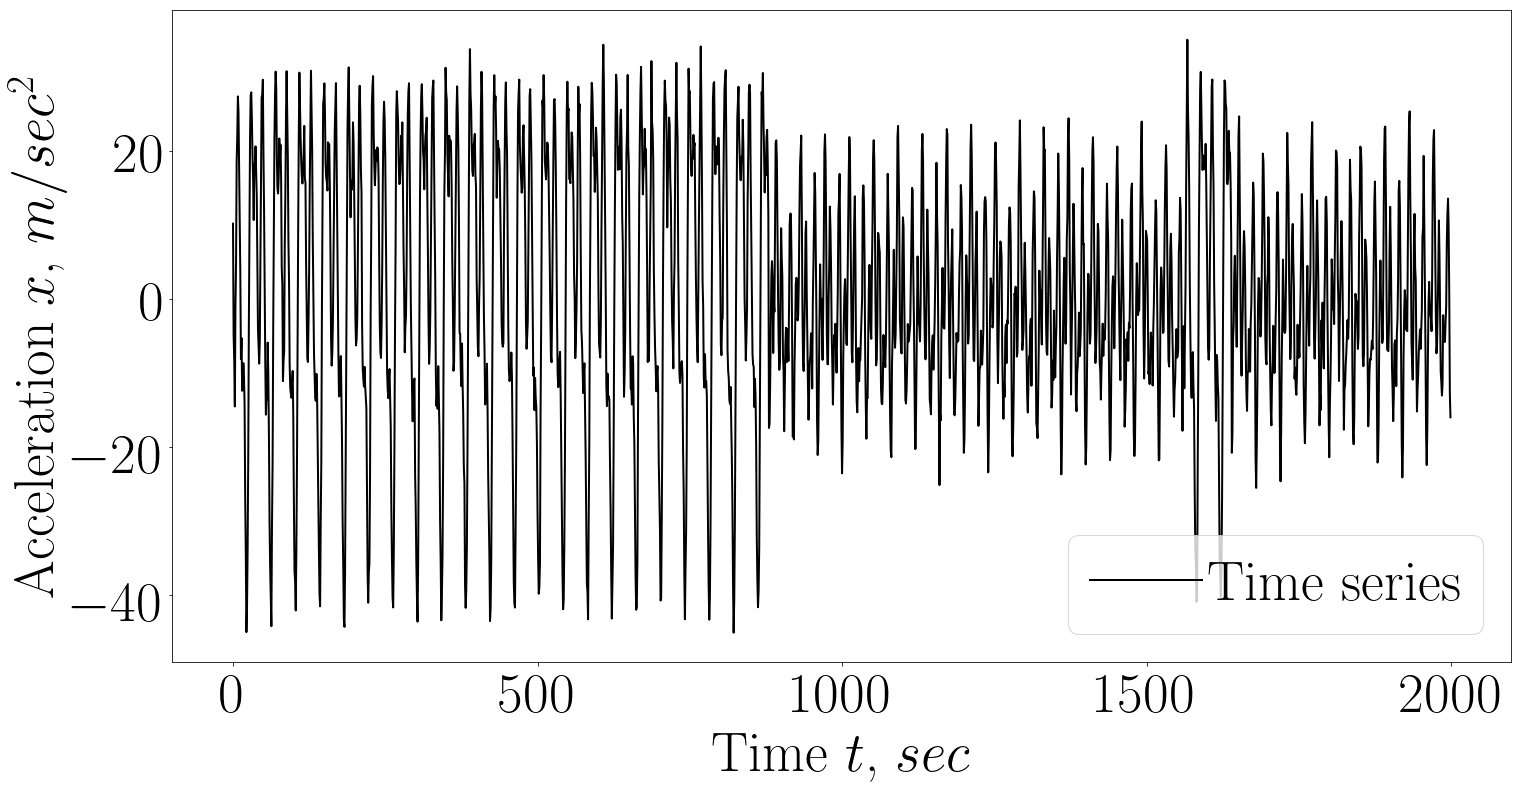
\includegraphics[width=0.5\textwidth]{results/2_patern_2_series}\label{fig_synthetic_series_2}}
\subfloat[]
{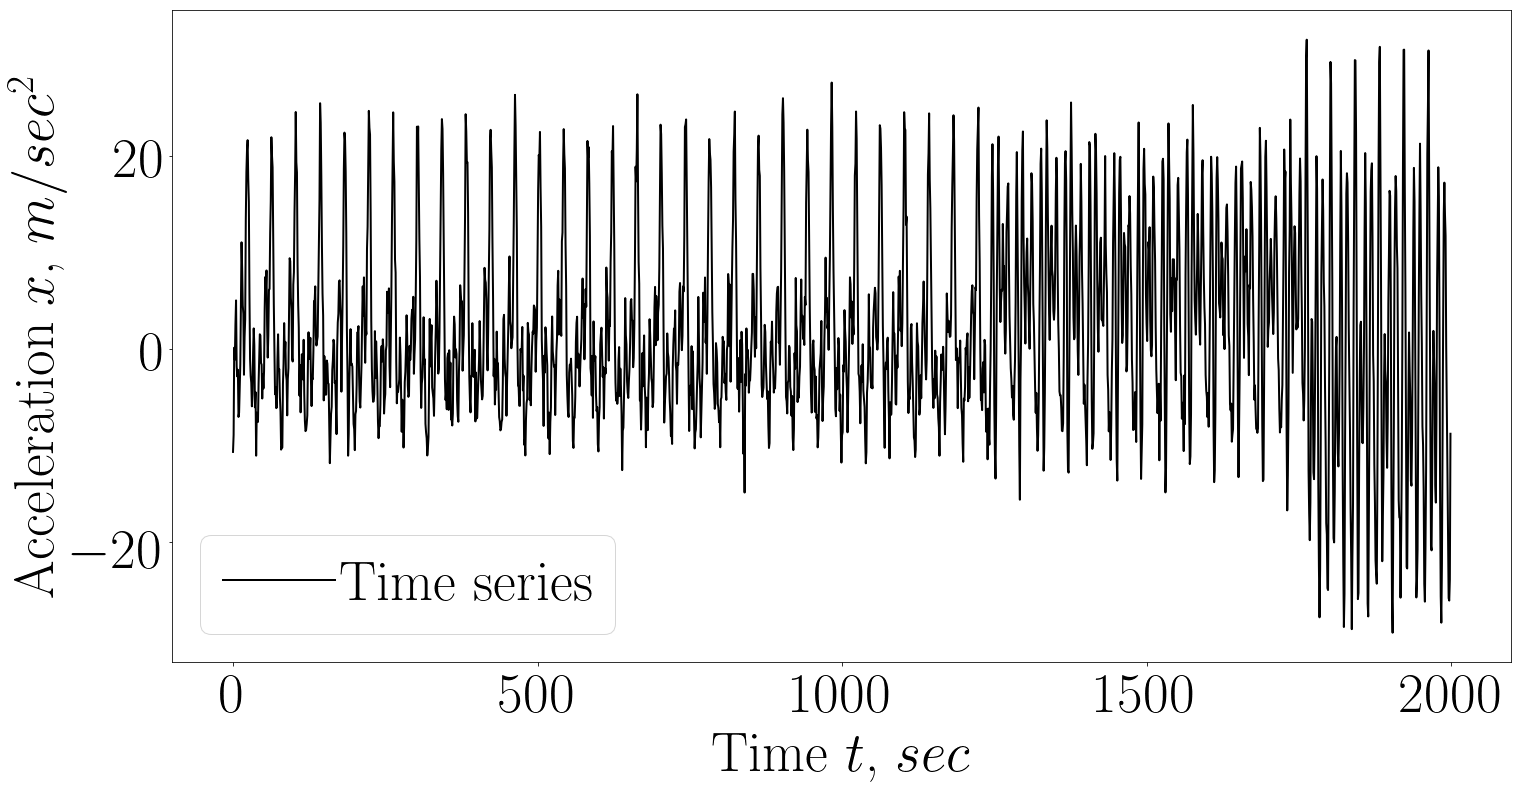
\includegraphics[width=0.5\textwidth]{results/3_patern_2_series}\label{fig_synthetic_series_3}}\\
\caption{Example of synthetic time series: a) Synthetic~1; b) Synthetic~2}
\label{fig_synthetic_series}
\end{figure}

\begin{figure}[h!t]\center
\subfloat[]
{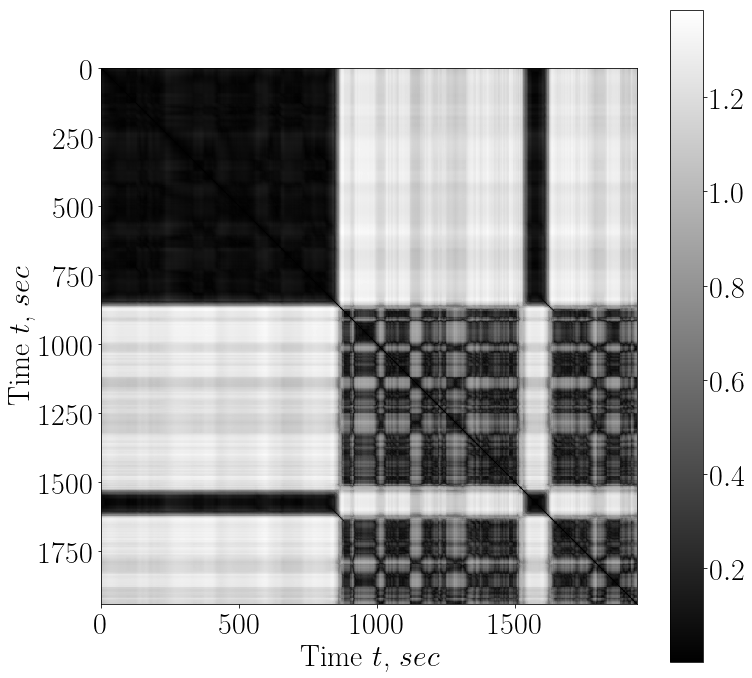
\includegraphics[width=0.5\textwidth]{results/2_patern_2_full}}
\subfloat[]
{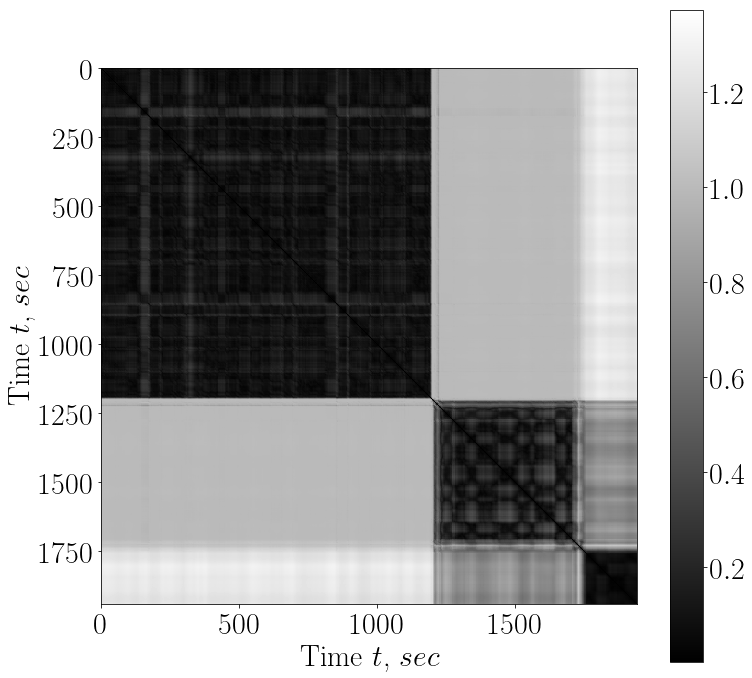
\includegraphics[width=0.5\textwidth]{results/3_patern_2_full}}\\
\caption{Pairwise distance matrix~$\textbf{M}$ between points of time series: a) Synthetic~1; b) Synthetic~2}
\label{fig_synthetic_distance}
\end{figure}

\begin{figure}[h!t]\center
\subfloat[]
{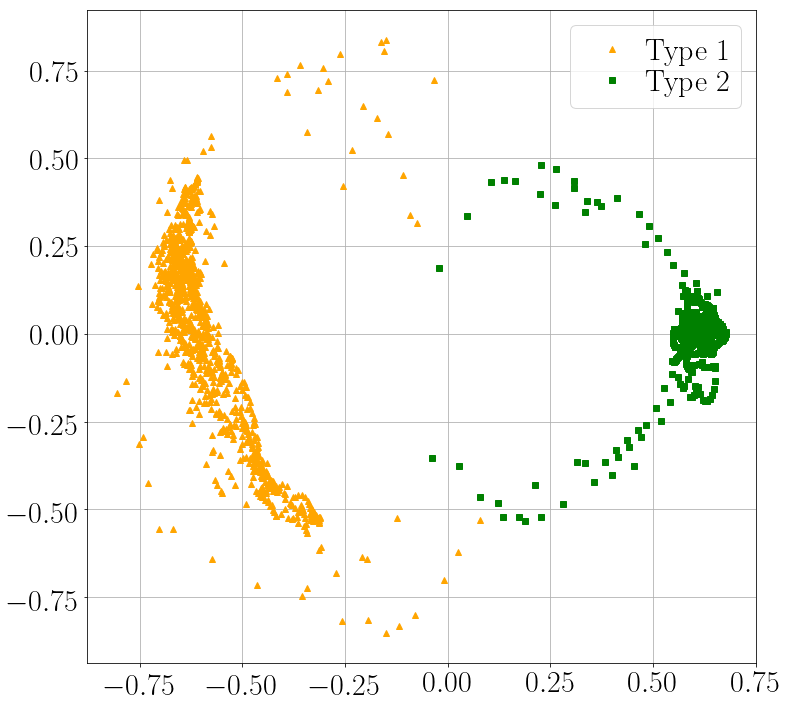
\includegraphics[width=0.5\textwidth]{results/2_patern_2_2D_vector}}
\subfloat[]
{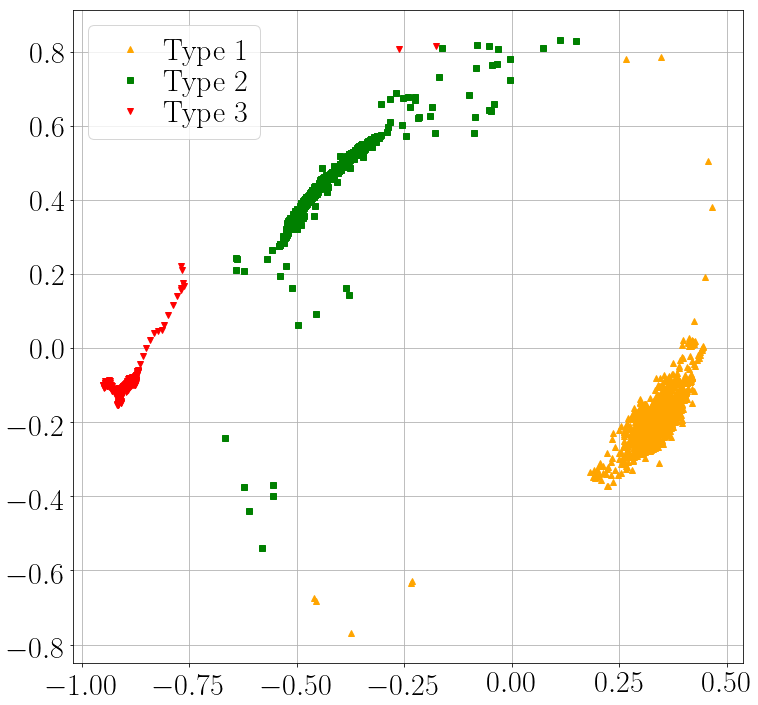
\includegraphics[width=0.5\textwidth]{results/3_patern_2_2D_vector}}\\
\caption{The projection of points on a plane by using the pairwise distance matrix~$\textbf{M}$: a) Synthetic~1; b) Synthetic~2}
\label{fig_synthetic_2D}
\end{figure}

\begin{figure}[h!t]\center
\subfloat[]
{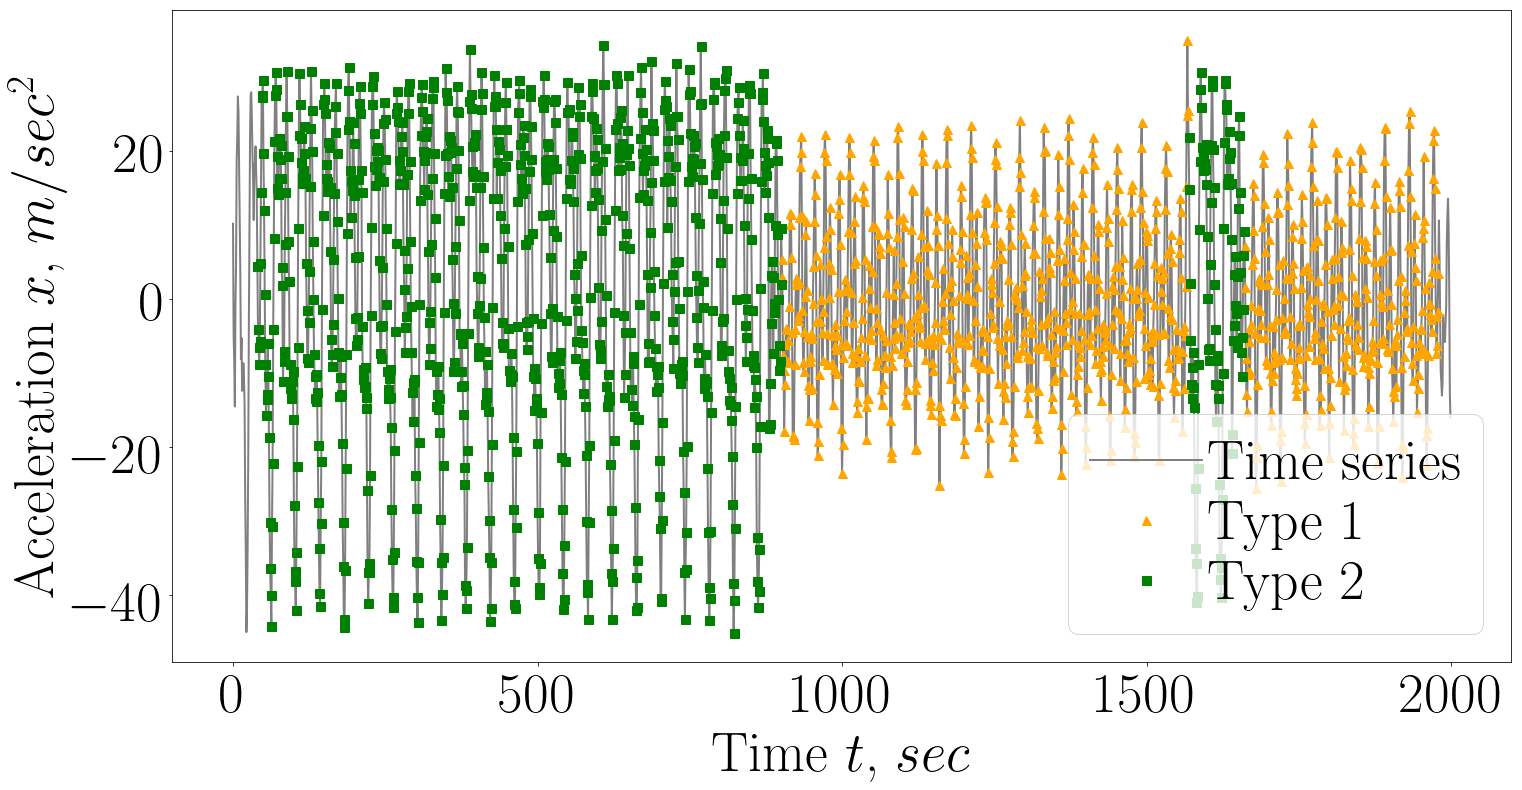
\includegraphics[width=0.5\textwidth]{results/2_patern_2_claster_vector}}
\subfloat[]
{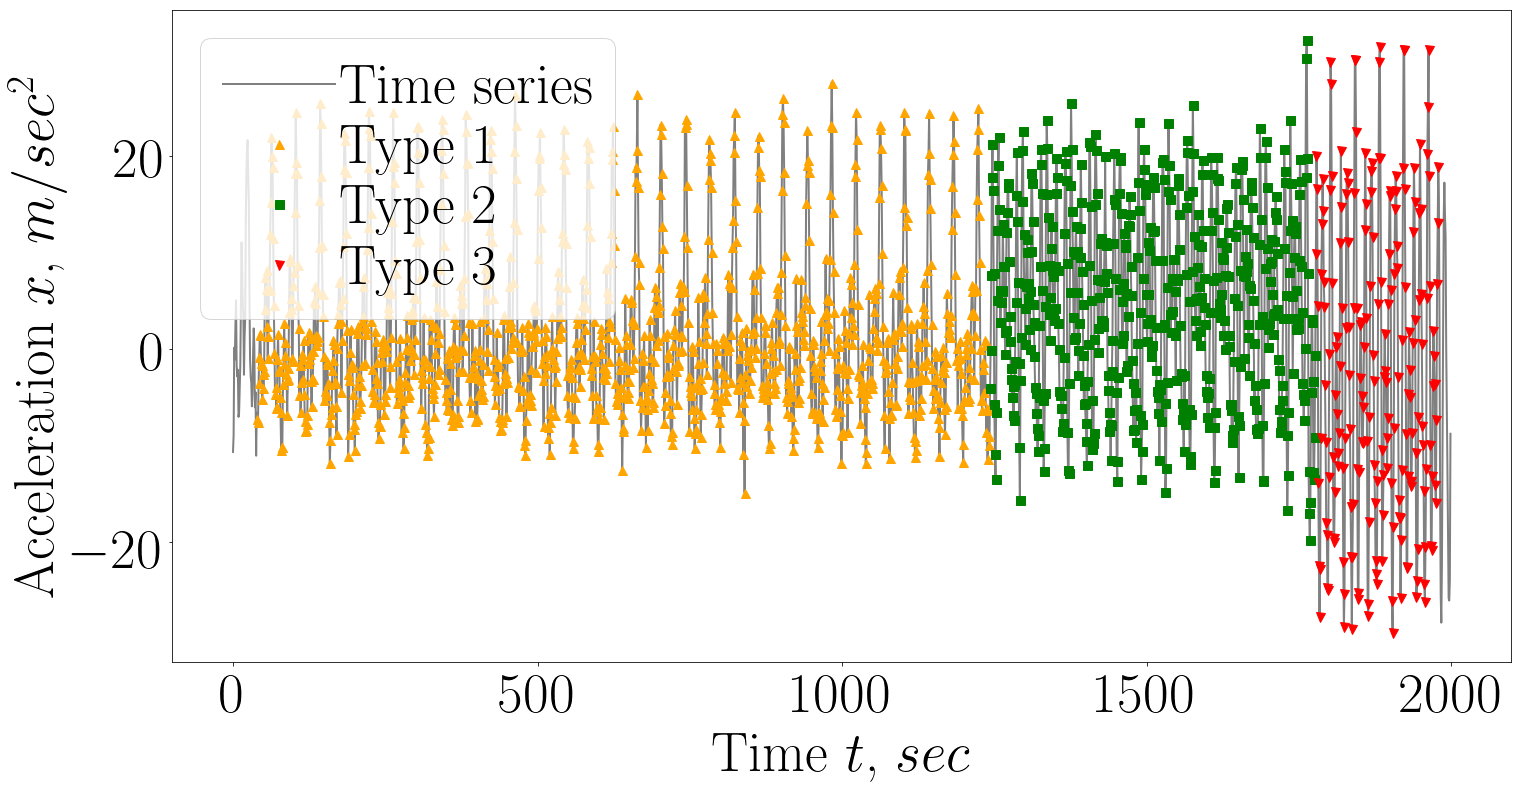
\includegraphics[width=0.5\textwidth]{results/3_patern_2_claster_vector}}\\
\caption{Time series points clustering: a) Synthetic~1; b) Synthetic~2}
\label{fig_synthetic_claster}
\end{figure}

\paragraph{Synthetic data.}

The fig.~\ref{fig_synthetic_series} shows an example of synthetic time series.
The fig.~\ref{fig_synthetic_series_2} shows an example of a time series in which the number of different segments is~$K = 2$, and the maximum length of segments is~$T = 20$.
The fig.~\ref{fig_synthetic_series_3} shows an example of a time series in which the number of different segments is~$K = 3$, and the maximum length of segments is~$T = 20$.

The fig.~\ref{fig_synthetic_distance} illustrates the pairwise distance matrix~$\textbf{M}$ between all pairs of points~$t$ in the time series, which are constructed by using equention~(\ref{eq:cl:9}).
Time series points can be easily visualized on a plane by using a pairwise distance matrix and a Multidimensional Scaling method~\cite{Borg2005}.
The fig.~\ref{fig_synthetic_2D} shows the visualization of points on the plane and performed their clustering by using the hierarchical clustering method.

\begin{figure}[h!t]\center
\subfloat[]
{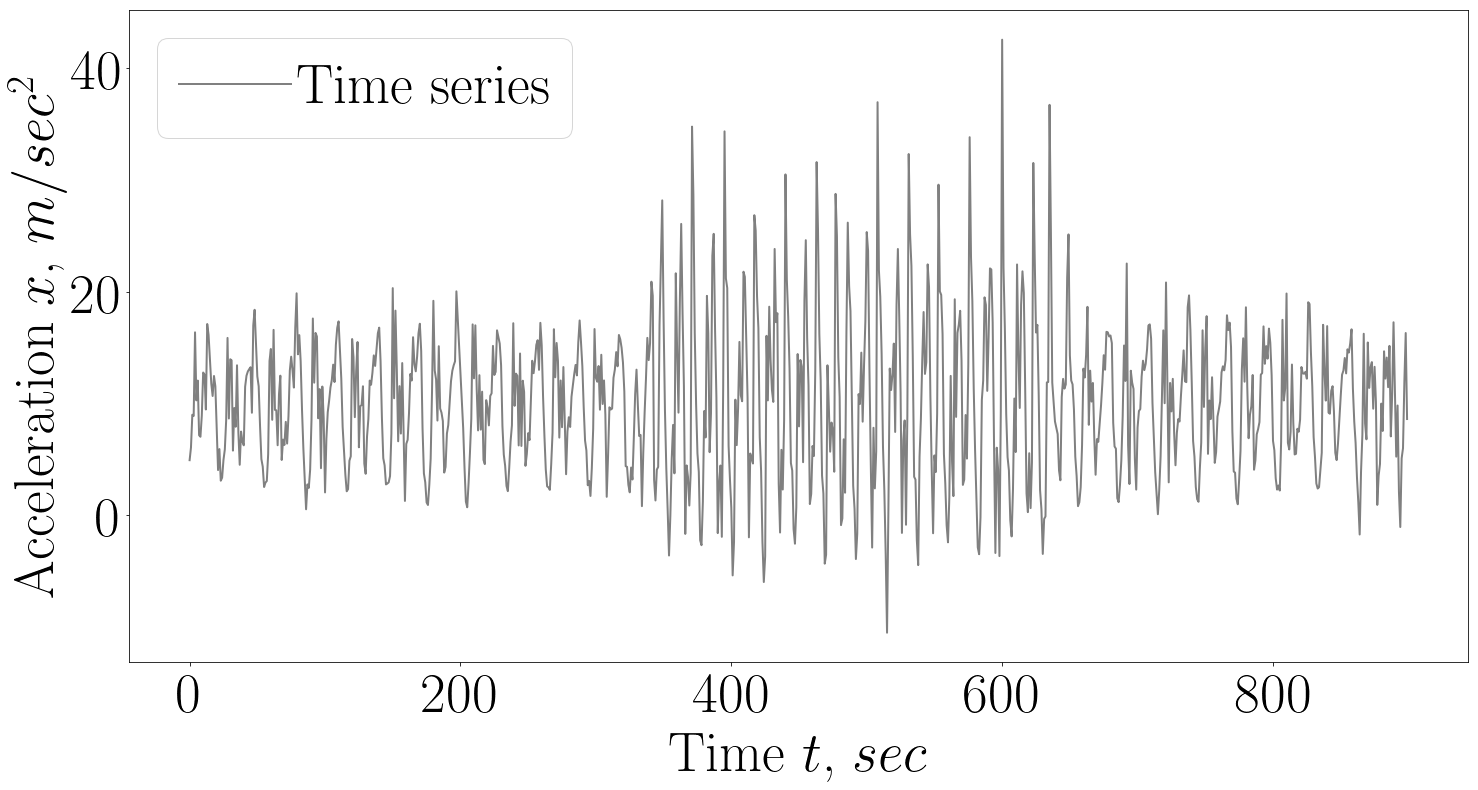
\includegraphics[width=0.5\textwidth]{results/real_1_series}}
\subfloat[]
{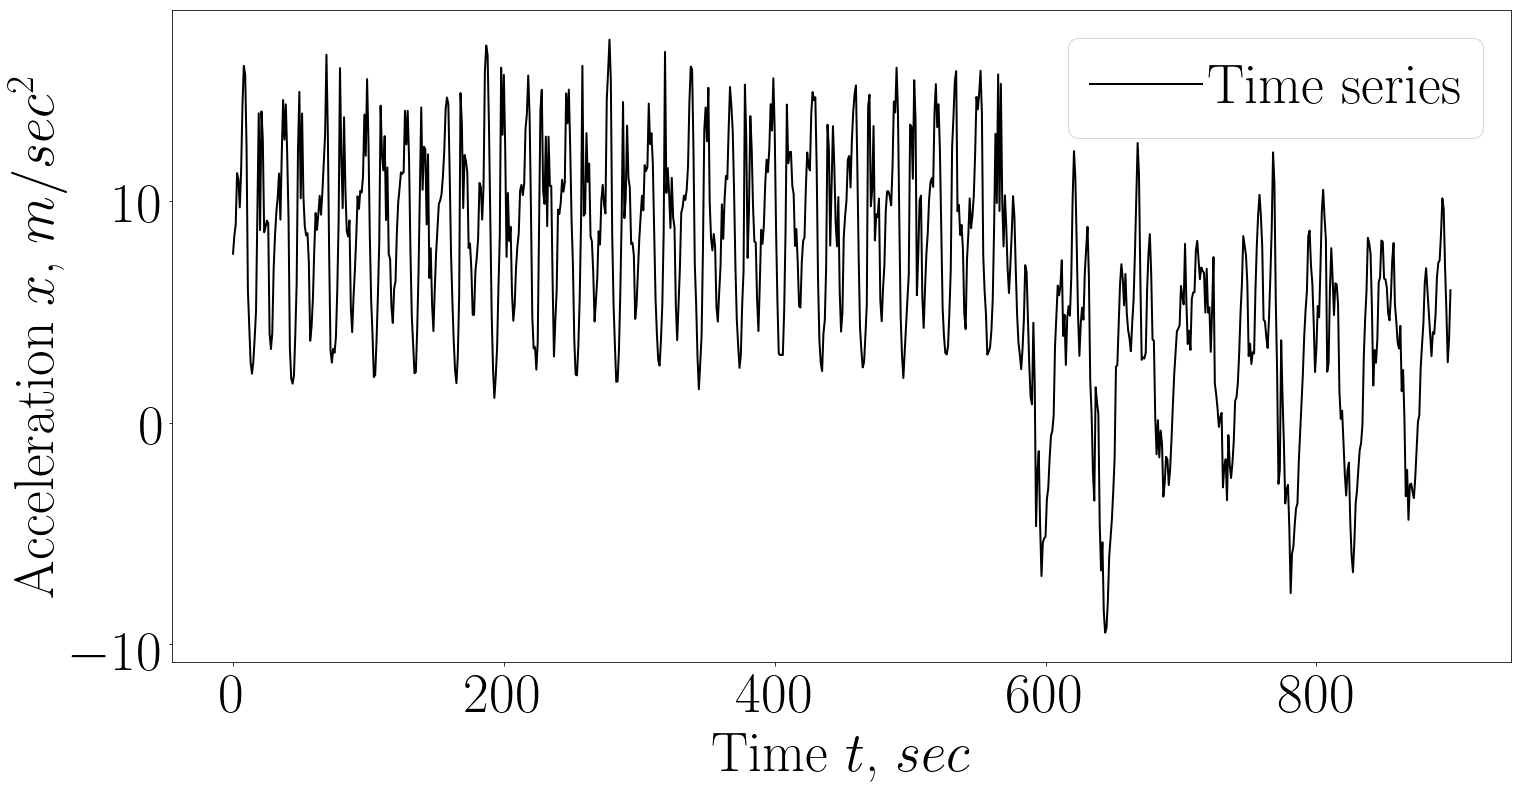
\includegraphics[width=0.5\textwidth]{results/real_2_series}}\\
\caption{Example of real time series: a) Physical~Motion~1; b) Physical~Motion~2}
\label{fig_real_series}
\end{figure}

\begin{figure}[h!t]\center
\subfloat[]
{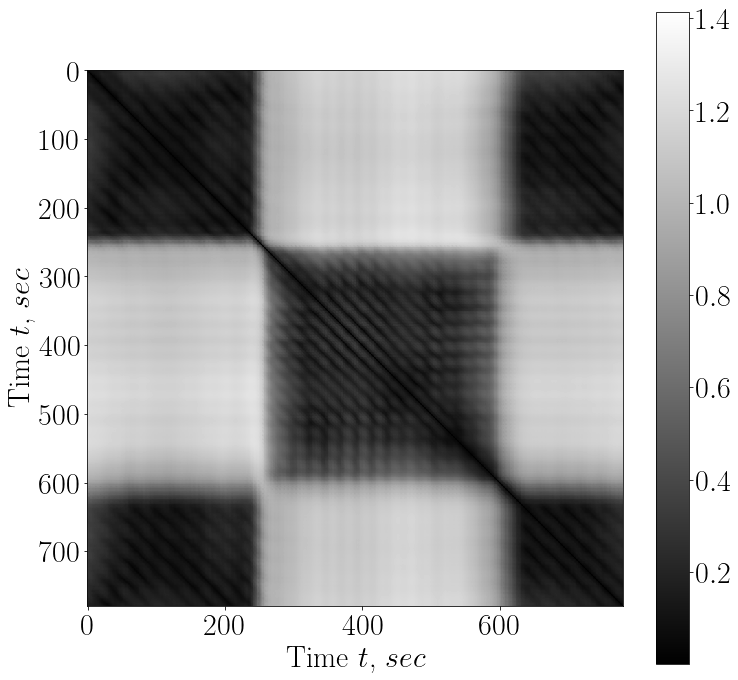
\includegraphics[width=0.5\textwidth]{results/real_1_full}}
\subfloat[]
{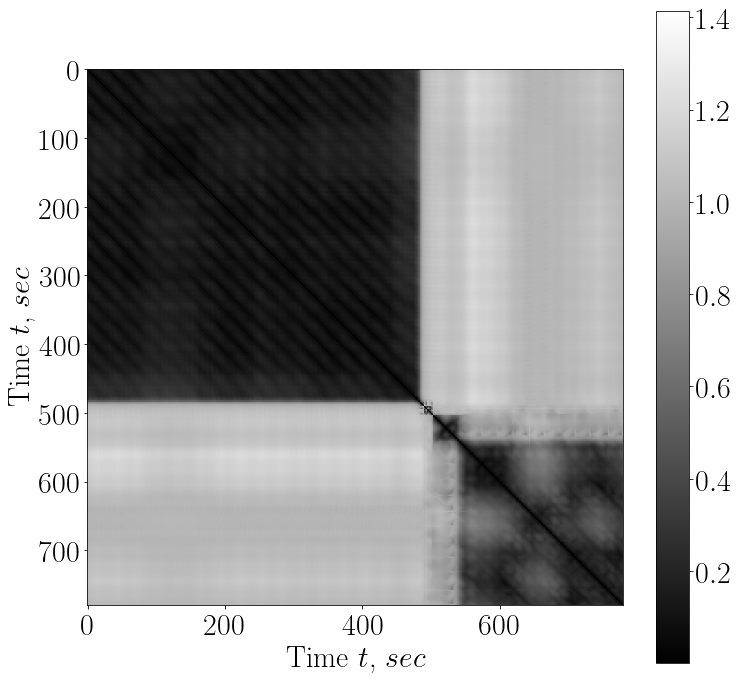
\includegraphics[width=0.5\textwidth]{results/real_2_full}}\\
\caption{Pairwise distance matrix~$\textbf{M}$ between points of time series:  a) Physical~Motion~1; b) Physical~Motion~2}
\label{fig_real_distance}
\end{figure}

\begin{figure}[h!t]\center
\subfloat[]
{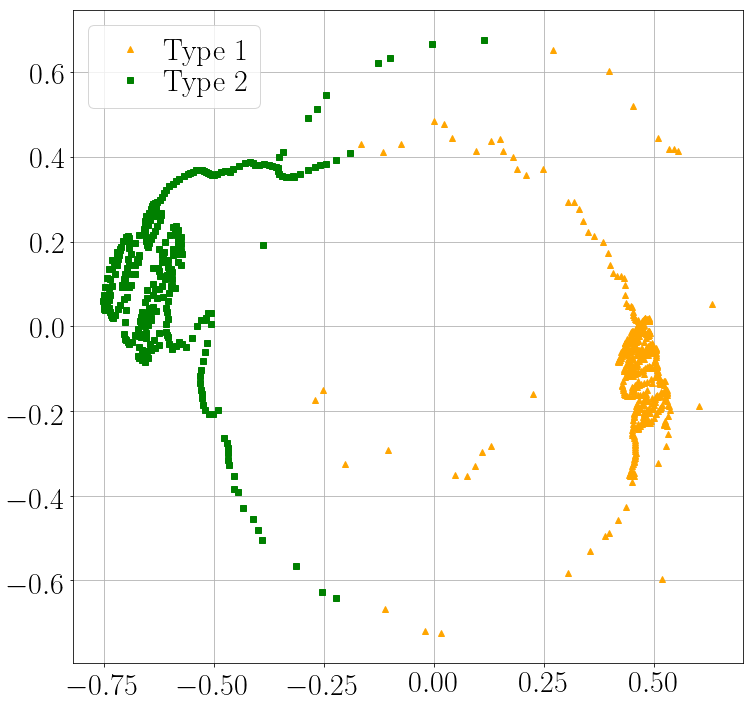
\includegraphics[width=0.5\textwidth]{results/real_1_2D_vector}}
\subfloat[]
{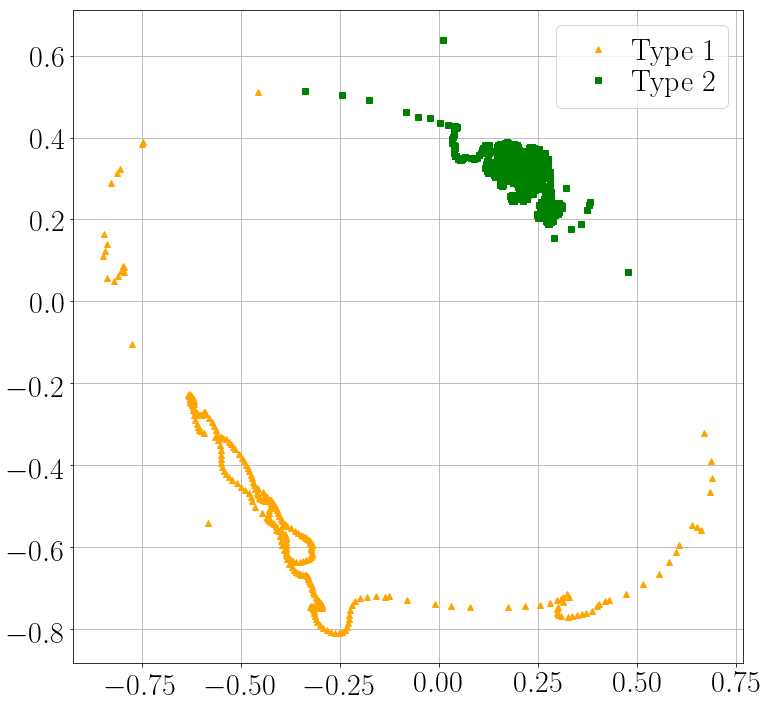
\includegraphics[width=0.5\textwidth]{results/real_2_2D_vector}}\\
\caption{The projection of points on a plane by using the pairwise distance matrix~$\textbf{M}$: a) Physical~Motion~1; b) Physical~Motion~2}
\label{fig_real_2D}
\end{figure}

\begin{figure}[h!t]\center
\subfloat[]
{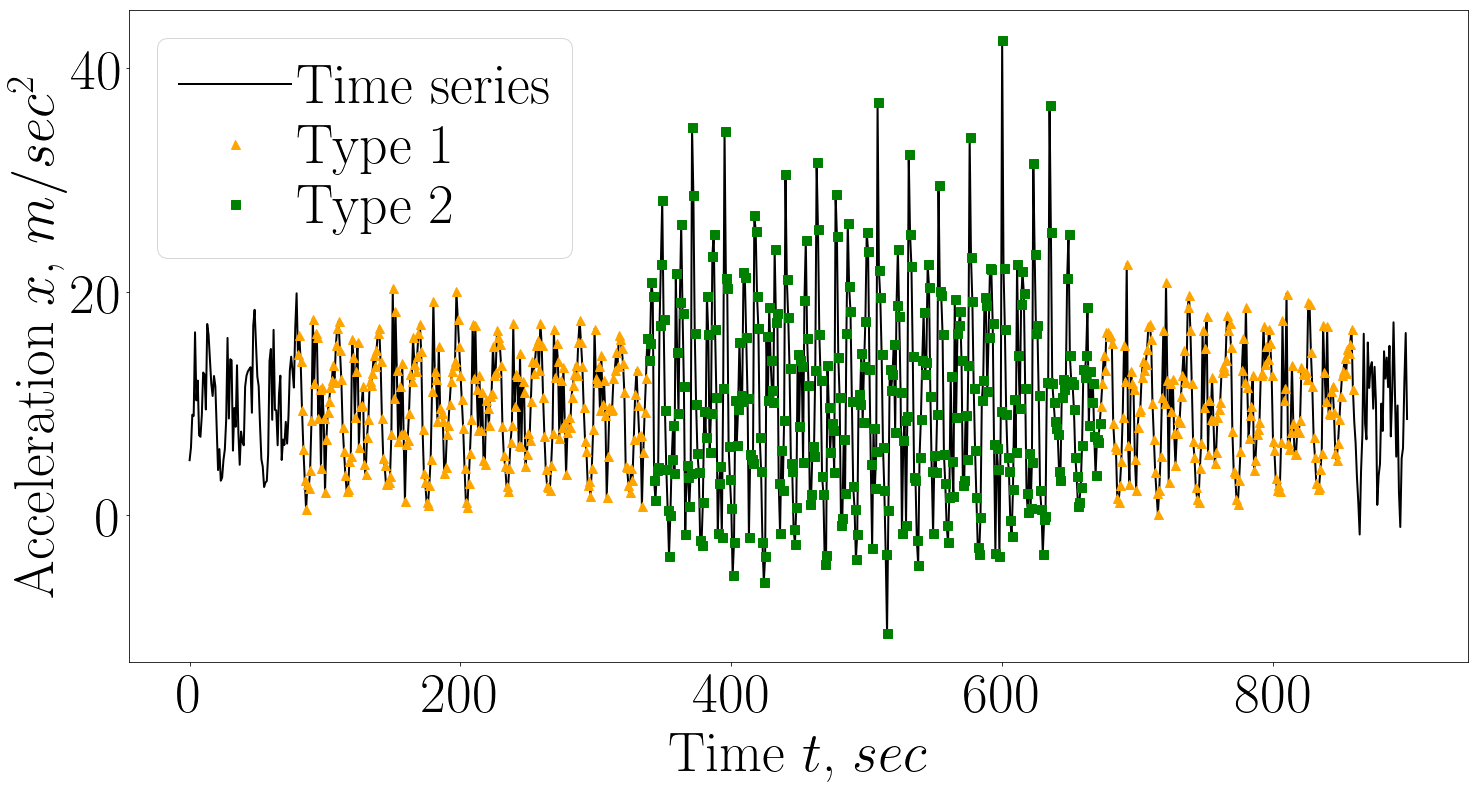
\includegraphics[width=0.5\textwidth]{results/real_1_claster_vector}}
\subfloat[]
{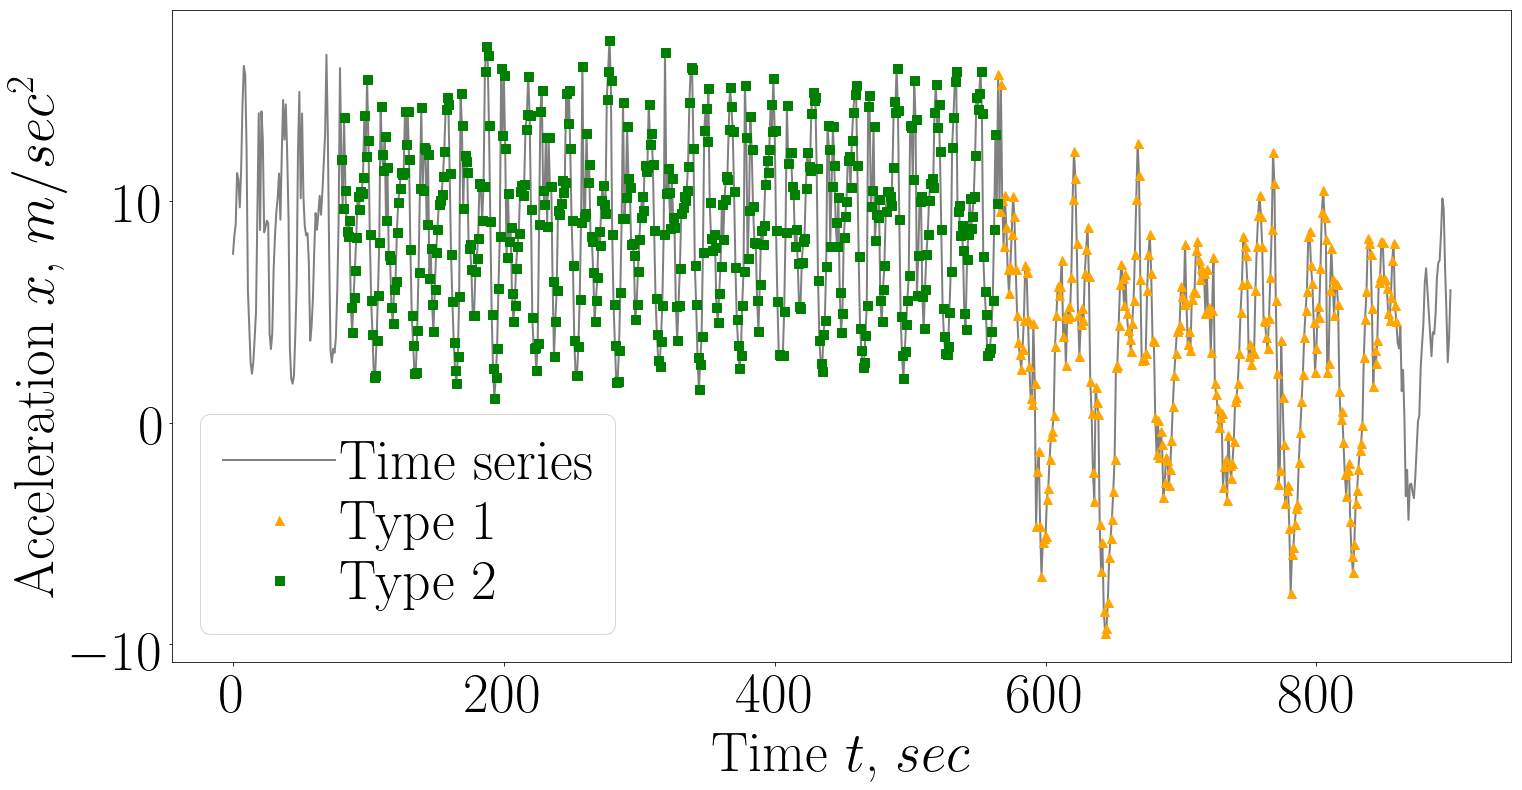
\includegraphics[width=0.5\textwidth]{results/real_2_claster_vector}}\\
\caption{Time series points clustering: 
a) Physical~Motion~1; b) Physical~Motion~2}
\label{fig_real_claster}
\end{figure}

\paragraph{Real data.}

The fig.~\ref{fig_real_series} shows an example of real time series obtained using a mobile accelerometer.

The fig.~\ref{fig_real_distance} illustrates the pairwise distance matrix~$\textbf{M}$ between all pairs of points~$t$ in the time series, which are constructed by using equention~(\ref{eq:cl:9}).
Time series points can be easily visualized on a plane by using a pairwise distance matrix and a Multidimensional Scaling method~\cite{Borg2005}.
The fig.~\ref{fig_real_2D} shows the visualization of points on the plane and performed their clustering by using the hierarchical clustering method.

\subsection{Time series segmentation}
Time series segmentation is carried out on synthetic and real data. 
A synthetic time series for this experiment were constructed by using the concatenation of two different sinusoidal signals with different amplitude and frequency.
The experiment was carried out on real and synthetic data, which are described in the table~\ref{table:3}.

Segmentation is carried out by using the method that is presented in the work~\cite{motrenko2015}. The method is used for each action within the time series separately.

\begin{table}[h!t]
\begin{center}
\caption{Description of time series in the experiment of segmentation}
\label{table:3}
\begin{tabular}{|c|c|c|c|}
\hline
	Series,~$\textbf{x}$ & Length,~$N$& Number of segments,~$K$& Period,~$T$\\
	\hline
	\multicolumn{1}{|l|}{Simple~1}
	& 1000& 2& 100\\
	\hline
	\multicolumn{1}{|l|}{Physical~Motion~2}
	& 900& 2& 40\\
\hline

\end{tabular}
\end{center}
\end{table}

\paragraph{Synthetic data.}
The fig.~\ref{fig_simple_segmentation} shows the result of the segmentation for the Simple~1 time series.
The algorithm is well marked the beginning of the segments.

The fig.~\ref{fig_simple_segmentation} shows the projections of the phase spaces for both clusters onto their first two main components.

\begin{figure}[h!t]\center
\subfloat[]
{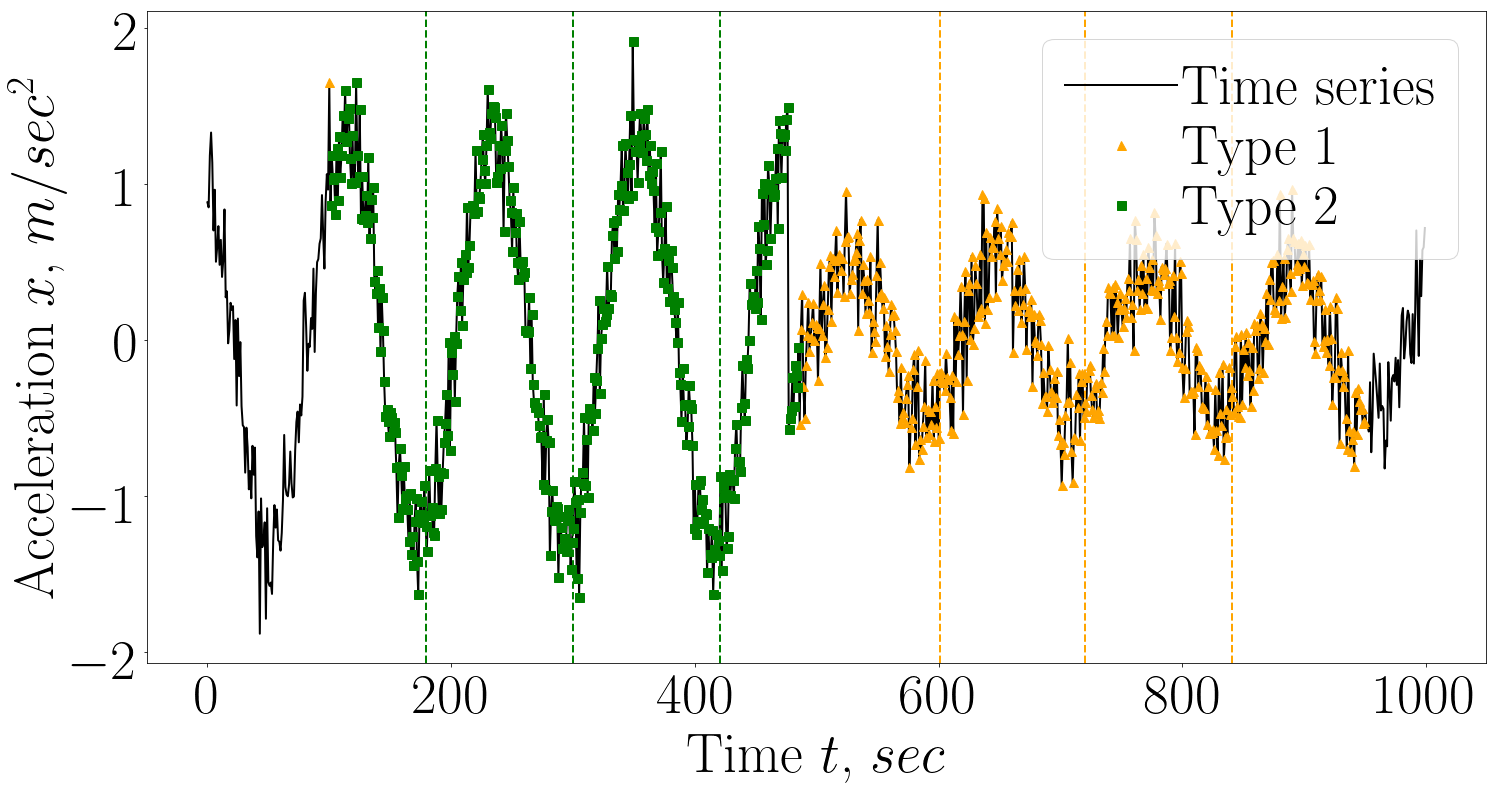
\includegraphics[width=0.5\textwidth]{results/simple_1_segmentation_vector}}
\subfloat[]
{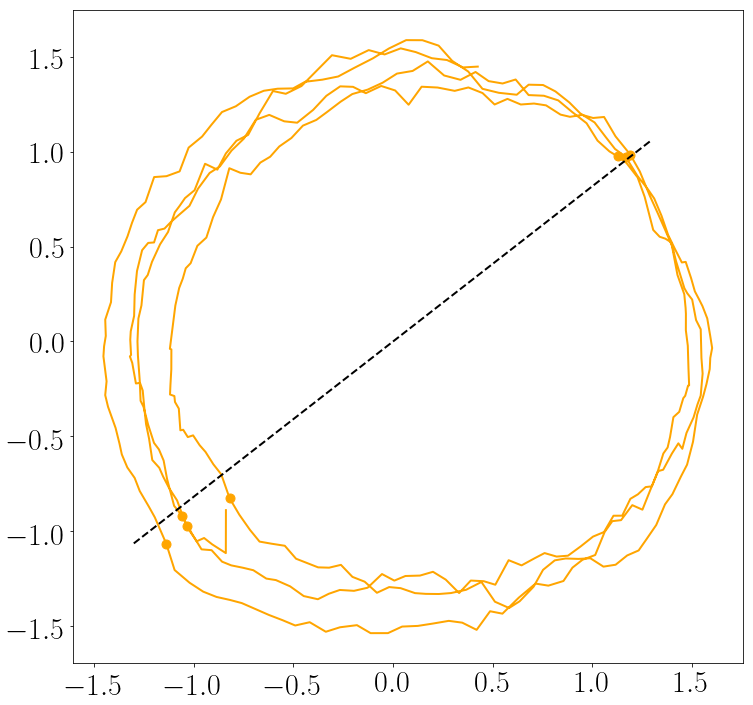
\includegraphics[width=0.25\textwidth]{results/simple_1_phase_space0}}
\subfloat[]
{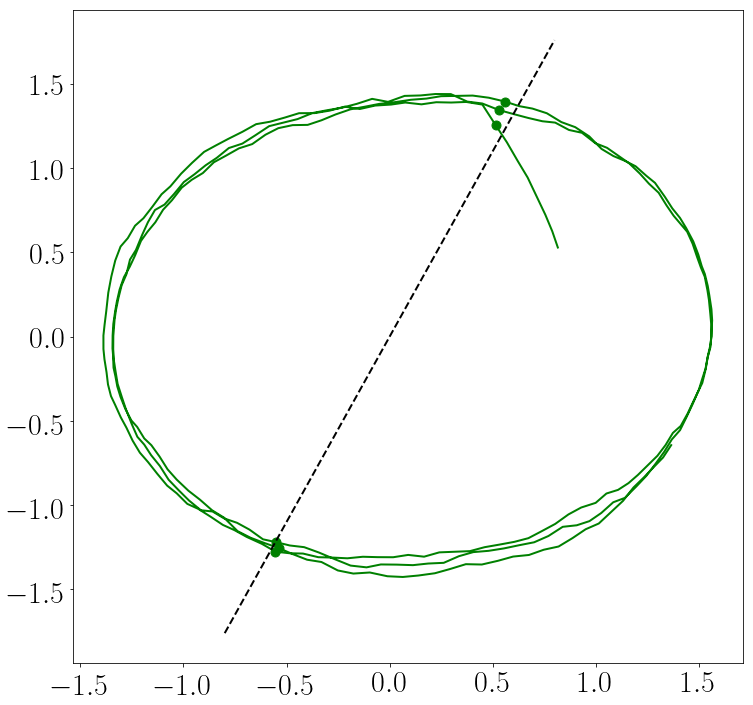
\includegraphics[width=0.25\textwidth]{results/simple_1_phase_space1}}\\
\caption{Segmentation for the Simple~1 time series: 
a) time series segmentation; b) the projection of the phase space on the first two principal components for the first cluster; c) the projection of the phase space on the first two principal components for the second cluster;}
\label{fig_simple_segmentation}
\end{figure}

\paragraph{Real data.}
The fig.~\ref{fig_simple_segmentation} shows the result of the segmentation for the Physical~Motion~2 time series.
The algorithm is well marked the beginning of the segments for Type~1 and bad for Type~2.
The fig.~\ref{fig_simple_segmentation} shows the projections of the phase spaces for both clusters onto their first two main components.
Bad segmentation was obtained due to self-intersection of the phase trajectory.

\begin{figure}[h!t]\center
\subfloat[]
{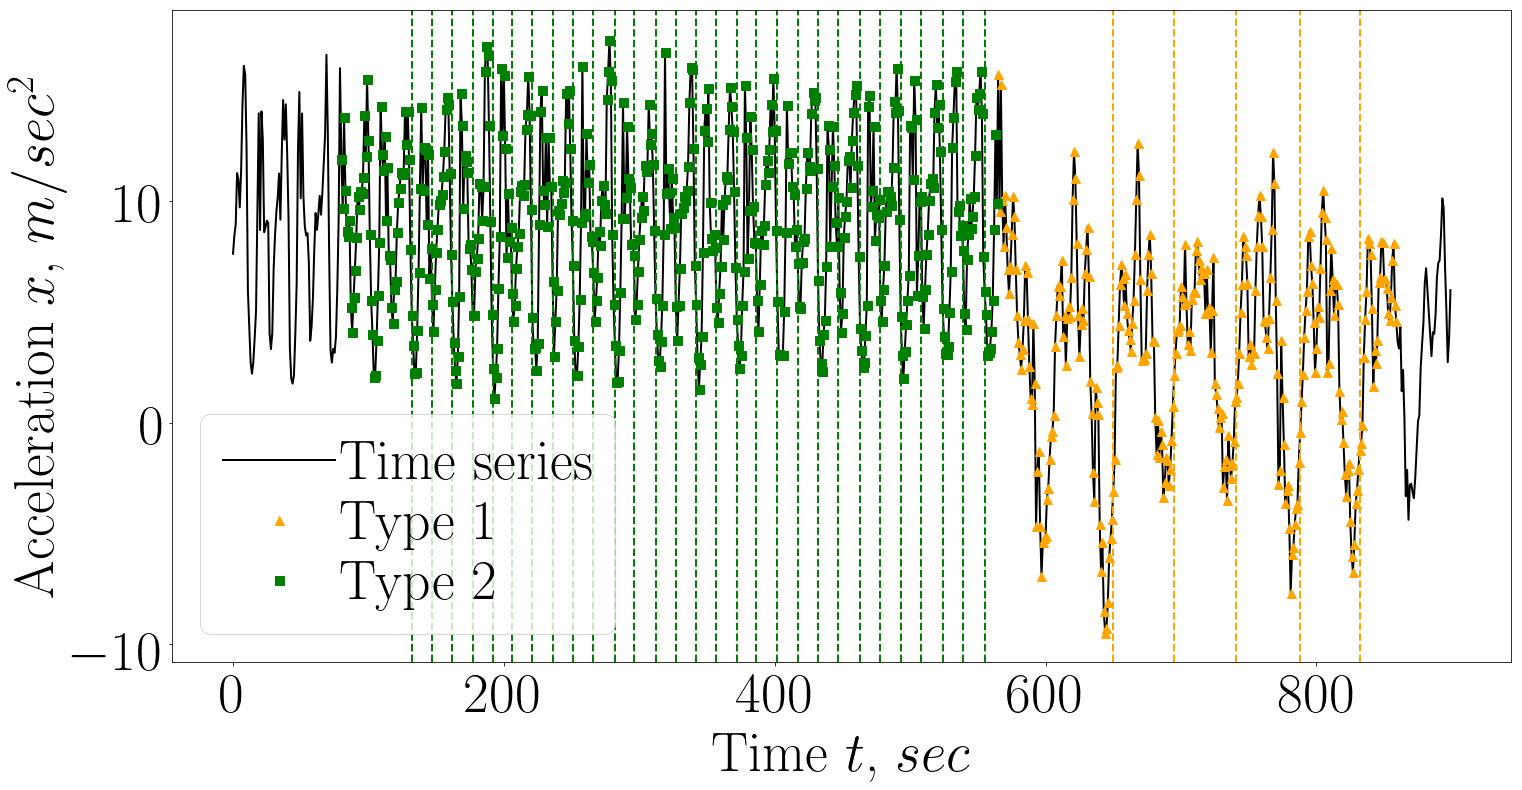
\includegraphics[width=0.5\textwidth]{results/real_2_segmentation_vector}}
\subfloat[]
{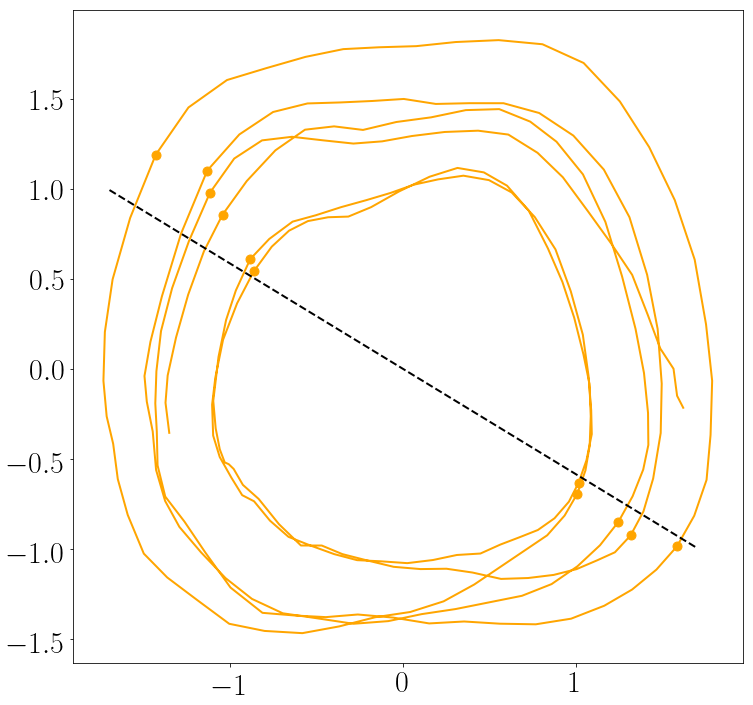
\includegraphics[width=0.25\textwidth]{results/real_2_phase_space0}}
\subfloat[]
{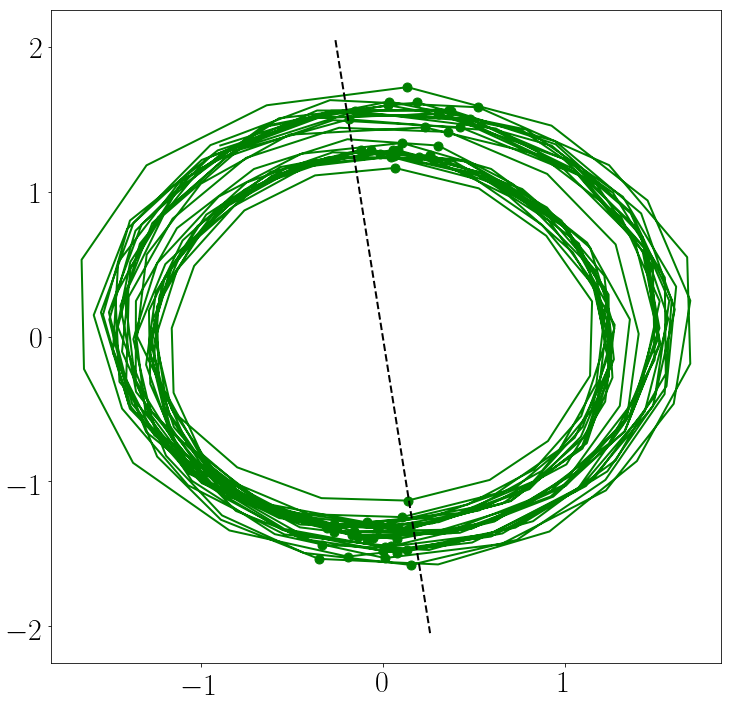
\includegraphics[width=0.25\textwidth]{results/real_2_phase_space1}}\\
\caption{Segmentation for the Physical~Motion~2 time series: 
a) time series segmentation; b) the projection of the phase space on the first two principal components for the first cluster; c) the projection of the phase space on the first two principal components for the second cluster;}
\label{fig_real_segmentation}
\end{figure}

\section{Conclusion}
\begin{table}[h!t]
\begin{center}
\caption{Algorithm analysis results}
\label{table_2}
\begin{tabular}{|c|c|c|c|c|}
\hline
	Series,~$\textbf{x}$ & Length,~$N$& Number of segments,~$K$& Period,~$T$& Error,~$S$\\
	\hline
	\multicolumn{1}{|l|}{Phys.~Motion~1}
	& 900& 2& 40& 0.06\\
	\hline
	\multicolumn{1}{|l|}{Phys.~Motion~2}
	& 900& 2& 40& 0.03\\
	\hline
	\multicolumn{1}{|l|}{Synthetic~1}
	& 2000& 2& 20& 0.04\\
	\hline
	\multicolumn{1}{|l|}{Synthetic~2}
	& 2000& 3& 20& 0.03\\
\hline

\end{tabular}
\end{center}
\end{table}

The paper considered the problem of finding periodic structures within a time series.
A method based on local reduction of the phase space dimension was considered.
An algorithm for searching for segments was proposed. 
The algorithm is based on the principal component method for local dimension reduction.
Also introduced is the function of the distance between local basis at each time instant. 
Local bases were interpreted as a features description of a point in the time series.

During the experiment on the real and synthetic data showed that the proposed method for measuring the distance between the basis well separates points that are related to different type of action, which leads to good clustering of time series points.
The results of the experiment are shown in the table~\ref{table_2}.
The experiment was carried out segmentation of time series by using the method~\cite{motrenko2015} for each cluster separately.

The proposed method has few disadvantages associated with a large number of assumption on a time series.
These restrictions will be relaxed in subsequent papers.
It is also planned to solve the problem of finding the minimum dimension of the phase space for which the phase trajectory will not have self-intersections.

\begin{thebibliography}{99}
	\bibitem{kwapisz2010}
	\textit{J. R. Kwapisz, G. M. Weiss, S. A. Moore} Activity Recognition using Cell Phone Accelerometers~// Proceedings of the Fourth International Workshop on Knowledge Discovery from Sensor Data, 2010. Vol. 12. P. 74--82.
	
	\bibitem{wang2014}
	\textit{W. Wang, H. Liu, L. Yu, F. Sun} Activity Recognition using Cell Phone Accelerometers~// Joint Conference on Neural Networks, 2014. P. 1185--1190.
	
	\bibitem{Ignatov2015}
	\textit{A. D. Ignatov, V. V. Strijov} Human activity recognition using quasiperiodic time series collected from a single tri-axial accelerometer.~// Multimedial Tools and Applications, 2015.
	
	\bibitem{Olivares2012}
	\textit{A. Olivares, J. Ramirez, J. M. Gorris, G. Olivares, M. Damas} Detection of (in)activity periods in human body motion using inertial sensors: A comparative study.~// Sensors, 12(5):5791–5814, 2012.
	
	\bibitem{cinar2018}
	\textit{Y. G. Cinar and H. Mirisaee} Period-aware content attention RNNs for time series forecasting with missing values~// Neurocomputing, 2018. Vol. 312. P. 177--186.
	
	\bibitem{motrenko2015}
	\textit{A. P. Motrenko, V. V. Strijov} Extracting fundamental periods to segment biomedical signals~// Journal of Biomedical and Health Informatics, 2015,~20(6). P.~1466~-~1476.
	
	\bibitem{lukashin2003}
	\textit{Y. P. Lukashin} Adaptive methods for short-term forecasting~// Finansy and Statistik, 2003.
	
	\bibitem{Ivkin2015}
	\textit{M. P. Kuznetsov,  N. P. Ivkin} Time series classification algorithm using combined feature description~// Machine Learning and Data Analysis, 2015,~11(1). P.~1471-1483.
	
	\bibitem{Katrutsa2015}
	\textit{V. V. Strijov, A. M. Katrutsa} Stresstes procedures for features selection algorithms.~// Schemometrics and Intelligent Laboratory System, 2015.
	
	\bibitem{Borg2005}
	\textit{I. Borg, P. J. F. Groenen} Modern Multidimensional Scaling. --- New York: Springer, 2005. 540 p.
	
	\bibitem{Shiglavsi1997}
	\textit{D. L. Danilov, A. A. Zhiglovsky} Main components of time series: method "Gesenitsa".~---~St.~Petersburg University, 1997.
	

	
\end{thebibliography}

\end{document}

